\documentclass{article}
\usepackage{tikz}
\usepackage{xcolor}

\definecolor{myblue}{RGB}{40,110,160}
\definecolor{bggray}{RGB}{240,240,240}
\definecolor{gridgray}{RGB}{180,180,180}

\begin{document}

\begin{center}
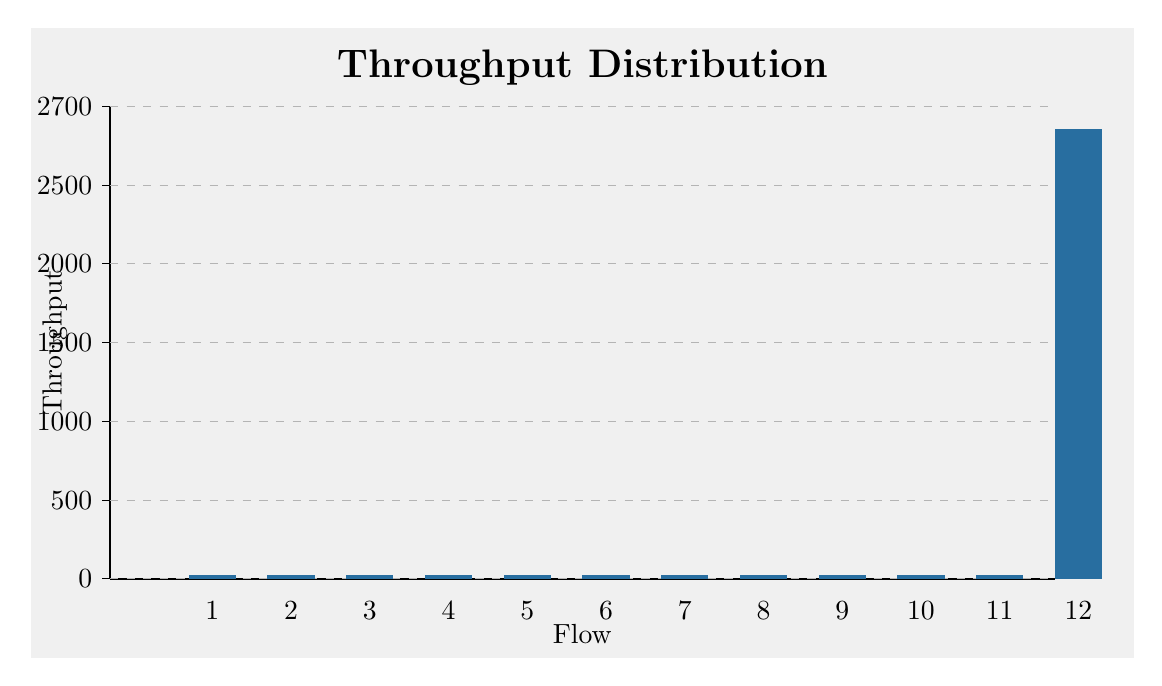
\begin{tikzpicture}

% Background
\fill[bggray] (0,0) rectangle (14,8);

% Axes
\draw[thick] (1,1) -- (1,7); % Y-axis
\draw[thick] (1,1) -- (13,1); % X-axis

% Title
\node[font=\Large\bfseries] at (7,7.5) {Throughput Distribution};

% Labels
\node[rotate=90] at (0.3,4) {Throughput};
\node at (7,0.3) {Flow};

% Y-axis scale (0 to 2700)
\foreach \y/\val in {
1/0,
2/500,
3/1000,
4/1500,
5/2000,
6/2500,
7/2700
} {
    \draw (0.9,\y) -- (1.1,\y);
    \node[left] at (0.9,\y) {\val};
    \draw[dashed, gridgray] (1,\y) -- (13,\y);
}

% Scaling factor
\def\scale{0.0022}

% Data values
\foreach \x/\val in {
1/20,2/22,3/21,4/23,5/22,6/24,
7/23,8/22,9/21,10/23,11/25,12/2600
} {
    \fill[myblue] (\x+1,1) rectangle (\x+1.6,{1 + \val*\scale});
}

% X-axis labels
\foreach \x in {1,...,12} {
    \node at (\x+1.3,0.6) {\x};
}

\end{tikzpicture}
\end{center}

\end{document}